\documentclass[12pt, report, a4paper, titlepage]{article}
\usepackage[left=3.5cm,right=3.5cm,top=2cm,bottom=3cm]{geometry}
\usepackage[utf8]{inputenc}

\title{Seedy Images: The SKIZ Operator and VOISE Algorithm for for Image Segmentation by Voronoi Diagrams}
\author{Jack Scantlebury \\ Department of Physics\\ University College London}
\date{2018}
\renewcommand{\baselinestretch}{1.6} 
\usepackage{fixmath}
\usepackage{placeins}
\usepackage{enumerate}
\usepackage{amsmath}
\numberwithin{equation}{section}
\usepackage{amsfonts}
\usepackage{braket,mleftright}
\mleftright
\usepackage{notoccite}
\newcommand\abs[1]{\left|#1\right|}
\usepackage[titletoc,toc]{appendix}
\usepackage[T1]{fontenc}
\usepackage[UKenglish]{babel}
\usepackage[version=3]{mhchem}
\usepackage{rsc}
\usepackage[font={small}]{caption}
\usepackage{blindtext}
\usepackage{titling}
\usepackage{graphicx} %package to manage images
\graphicspath{{images/}}
\usepackage{subcaption}
\usepackage[rightcaption]{sidecap}
\usepackage{float}
\usepackage{wrapfig}
\usepackage{blindtext}
\usepackage{caption}
\usepackage{textcomp}
\usepackage{amsmath} % or simply amstext
\usepackage{mathtools}
\usepackage{physics}
\newcommand{\angstrom}{\textup{\AA}}
\renewcommand{\arraystretch}{1.25}
\captionsetup{
  font=footnotesize,
  labelfont=bf,
  tableposition=top
}
\usepackage{fancyhdr}
\pagestyle{fancy}
\lhead{}
\chead{}
\rhead{}
\lfoot{}
\rfoot{}
\cfoot{Page \thepage}
\renewcommand{\headrulewidth}{0pt}
\renewcommand{\footrulewidth}{0.4pt}
\newcommand*{\citen}{}% generate error, if `\citen` is already in use
\DeclareRobustCommand*{\citen}[1]{%
  \begingroup
    \romannumeral-`\x % remove space at the beginning of \setcitestyle
    \setcitestyle{numbers}%
    \cite{#1}%
  \endgroup
}

\begin{document}
\maketitle

\newpage
\tableofcontents
\newpage
\thispagestyle{fancy}

\begin{abstract}
    **WRITE ABSTRACT: BRIEF SUMMARY OF PROJECT AND RESULTS**
\end{abstract}

\section{Summary of Achievements}

It has been impressed upon the students on this course that it should be clear what has been achieved over the course of each project. In the spirit of this, and in the interests of clarity, these are briefly  summarised as follows:

\begin{enumerate}
	\item A robust, efficient C++ implementation of the SKIZ operator algorithm as defined in [\citen{skiz}], along with appropriate MEX Matlab bindings for extremely fast computation of discrete Voronoi diagrams
	\item Extensive benchmarking of the SKIZ operator in its MEX binary form, compared with previous incremental and 'full' Voronoi diagram implementations. Improvements of between 18 and 105 times over previous incremental implementation and up to 10,000 times over 'full' native Matlab Qhull Voronoi diagram implementation
	\item Incorporation of SKIZ MEX binaries into the existing VOISE algorithm Matlab code [\citen{VOISE}]
	\item Profiling of existing VOISE code and conversion to C++ MEX of other bottleneck functions
	\item Application of VOISE algorithm to images collected by Hubble space telescope of Jovian magnetosphere, including cluster analysis and other machine learning techniques.
\end{enumerate}
\section{Voronoi Diagrams: A Crash Course}

While the concept of a Voronoi diagram (VD) was present as long ago as the 17$^{th}$ century, a mathematically rigorous definition and formalisation of the the general case is credited to Ukrainian mathematician Georgy Voronyi in 1908 \citen{Voronoi1908}. In loose terms, a VD can be summarised as a space in n dimensions which has been split into different 'Voronoi regions' (VRs). Coordinates in the same VR are closer, according to some valid distance measure, to the same 'feature point' or seed $s$ than any other seed in the space. The boundary of these VRs is the VD. An example of a VD in $\mathbb{R}^2$ which uses Euclidian distance can be seen in Fig. \ref{simple-vd}.

\begin{figure}[h!]
	\center
 	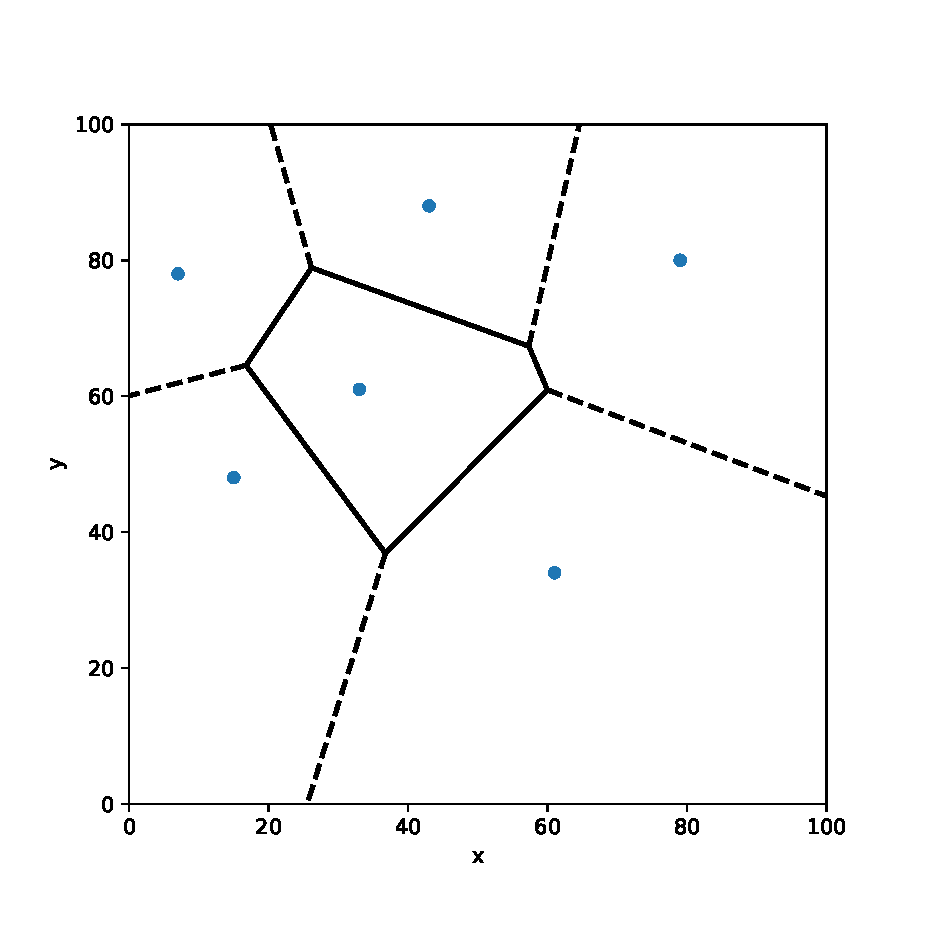
\includegraphics[width=.9\linewidth]{voronoi-simple.eps}
    \caption{A simple Voronoi diagram in $\mathbb{R}^2$. Dots are seeds, dashed lines are half lines and solid lines are lines.}
    \label{simple-vd}
\end{figure}

The seeds on the outside of the diagram are in unbounded, infinitely large VRs, and the lines that separate these are half-lines. The set of all seeds of this type form the convex hull $P$ of the set of all seeds $S$ (so $P \subseteq S$). The only fully enclosed VR in this case is in the middle.

More formally, the VR of a seed $\mathcal{R}(s)$ is defined in any metric space $M$ with associated distance function $d$ as:
\begin{align} \label{eq:1.1}
	\mathcal{R}(s) &= \underset{r \in S\textbackslash s}{\bigcap} \{ p \in M : d(p, s) < d(p, r) \} 
\end{align}
The edge between two neighbouring VRs is then:
\begin{align}
	\partial\mathcal{R}(s) \cap \partial\mathcal{R}(r) &= \underset{t \in S\textbackslash\{ r, s \}}{\bigcap} \{ p \in M : d(p, s) = d(p, r) \leq d(p, t) \} 
\end{align}
Finally, the VD is composed of the edges:
\begin{align}
	\mathcal{V}(S) &= \underset{\begin{subarray}{c}
  r, s \in S \\
  s \neq r
  \end{subarray}}{\bigcup} \left ( \partial\mathcal{R}(s) \cap \partial\mathcal{R}(r) \right )
\end{align}
Equation \ref{eq:1.1} defines a half plane if Euclidian distance is used. $\mathcal{R}(s)$ is the intersection of half planes, which are themselves convex sets, so $\mathcal{R}(s)$ is a convex set. A proof for $\mathbb{R}{^2}$ can be found in [\citen{skiz}], proposition 1.

\subsection{Delaunay Triangulation}

The dual $\mathcal{V}(S)$ is a Delaunay triangulation (DT or $\mathcal{D}(S)$). In $\mathbb{R}{^2}$, a DT is the triangulation of a set of points such that no point in the set lies in the circumcircle of any triangle in the triangulation. The points here are the seeds in the VD. A DT maximises the smallest angle, avoiding extremely thin triangles. This can be generalised to an arbitrarily high dimension; an example of a DT is shown in Fig. \ref{simple-dt}.

\begin{figure}[h!]
	\center
 	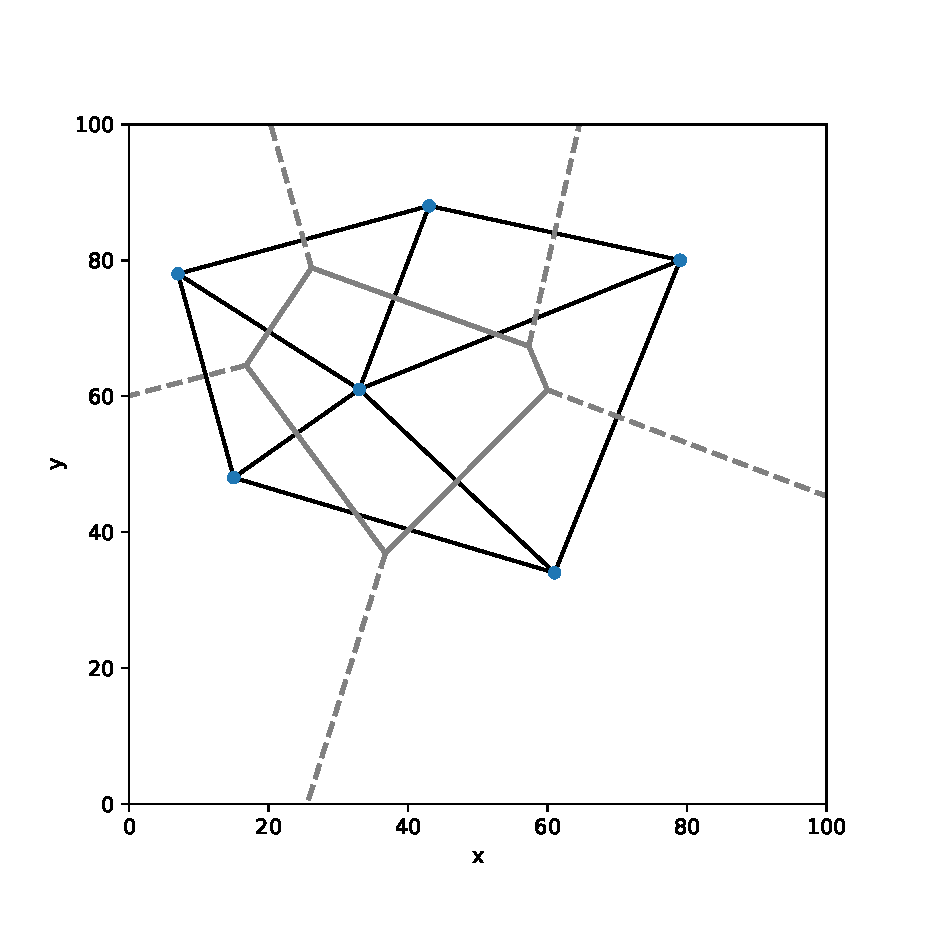
\includegraphics[width=.9\linewidth]{voronoi-simple-delaunay.eps}
    \caption{Voronoi diagram (gray) and Delaunay triangulation (black) in $\mathbb{R}^2$. Seeds are blue circles.}
    \label{simple-dt}
\end{figure}

Connecting the circumcentres of neighbouring triangles in $\mathcal{D}(S)$ recovers $\mathcal{V}(S)$; in this way, knowledge of one representation can be used to find the other.

\subsection{Degenerate Conditions}

The above discussion about Delaunay triangulations leads naturally to the problem of degenerate seed configurations. It should be noted that when working in a restricted space, as we must when dealing with images made up of a finite number of pixels, the probability of observing these conditions grows from infinitessimal to improbable. The two classes that must be handled by any robust algorithm are cocirulcarity and colinearity, neither of which are trivial obstsacles and both of which are dealt with in later chapters. For now, definitions will suffice.

\subsubsection{Cocircularity}

$\mathcal{D}(S)$ is only a unique triangulation if there are precisely three seeds on the circumcircle of each triangle. If there are $n$ cocircular points, there is no unique local (and therefore global) solution. In fact, there are ${n\choose 3}$ triangles that could be formed.

\subsubsection{Collinearity}

If three or more neighbouring seeds form a straight line, there is no $\mathcal{D}(S)$ because it not possible to form a circumcircle. In this circumstance, $\mathcal{V}(S)$ still exists, although most algorithms (including Fortune's Algorithm) do not handle this eventuality.

\section{Motivation}

Voronoi diagrams are well-studied, and have found applications in almost every quantitative field. In computational chemistry, VDs in $\mathbb{R}^3$ - where the diagram is defined by the location of the nuclei - can be used to model charge distribution in molecules [\citen{chem_voronoi}] and in crystallography, Weigner-Seitz cells and the space packing of metallic lattices can be modelled in a similar fashion. In biology, they can be used to model the growth of rival colonies of cells, the growth patterns of forests and the growth of bone tissue. They are used in engineering for finding triangulations that avoid small angles in finite element analysis [\citen{shontz_2010}], as well as in anthropology, cartography, robotics, geography, metallurgy and meteorology.

Of course, the particular interest here the use of VDs in astronomy. The 'cellular structure of the universe' is explored in [\citen{zaninetti_2006}], where VDs are used to expain the distribution of cosmological entities, and the size of the voids found between them. In [\citen{ramella_2001}], a VD is defined by the galaxies in images taken by telescopes, and the VD is used to build a picture of larger structures such as clusters. Other work in this area can be found in [\citen{ikeuchi_turner_1991}] and [\citen{ryden_1995}].

The work in this project builds on work in two papers: the VOISE algorithm [\citen{VOISE}] and the SKIZ Operator algorithm [\citen{skiz}]. We shall outline the former, and explain the utility of the latter in its efficient implementation.

\subsection{The VOISE Algorithm}

The VOronoi Image SEgmentation algorithm (VOISE) is a self-regulating, iterative method for image segmentation - that is, the partitioning of images into regions $\mathcal{R}(s)$ where pixels in the same region are similar according to some measure (pixel intensity, for example). A segmented image has a number of advantages as a representation over its original source, some of which will become clear in the following discussion.

While VDs can be defined in arbitrary dimensions, for this discussion, we are working in what can be best described as 'pixel-space'. This is $\mathbb{R}^2$ restricted to integer values between zero and some maximum, defined by the resolution of the image. In [\citen{skiz}], this this space is denoted by $W$, but here as in [\citen{VOISE}], we shall call it $\Omega$. All seeds $s$ and regions $\mathcal{R}(s)$ are only defined in $\Omega$, such that $\mathcal{R}(s_i)$ is all of the pixels in the Voronoi region defined by seed $s_i$.

There are four stages to VOISE: initialise, divide, merge and regularise. Initialisation begins the process with a random distribution of seeds and an initial VD; in the dividing phase, Voronoi seeds are added to the image according to the measure homogeneity found in each Voronoi region. In the merging phase, neighbouring regions which are similar are merged, in order to remove excessive granularity of the resulting representation. In third and final stage, the seed positions which cause the often irregularly shaped tiles from the first two stages are changed, resulting in a more regular tesselation.

\subsubsection{Initialisation}

In order to be able to evaluate intra-cellular homogeneity, some initial VD must be generated which does not make any assumptions on the underlying structures to be extracted. Seed generation under a uniform distribution over a bounded region is a binomial point process. We then calculate the VD for those seeds, restricted to $\Omega$, after which we can use information from the pixels in the raw image to better inform our placement of seeds in subsequent iterations.

\subsubsection{Division}

Most of the useful information to be extracted by VOISE is generated in this, the second and most important phase. After the initial distribution of seeds, each $\mathcal{R}(s_i), s_i \in S$ has associated with it a set of pixels in its region. The tile associated with each seed can then be filled according to some criterion, for example the median pixel value, to generate the representation at each iteration.

In order to continue creating cells in areas of heterogeneity, the homogeneity of a Voronoi region associated with seed $s_i$ is defined:
\begin{align}
\label{homogeneity}
	\chi(\mathcal{I}, s_i) &= \frac{\max_{p \in \mathcal{R}(s_i)} [\mathcal{I}(p)] - \min_{p \in \mathcal{R}(s_i)} [\mathcal{I}(p)]}{\left|\left|\chi (\mathcal{I}, S) \right|\right|_\infty}
\end{align}

where $\mathcal{I}$ is the image, $\chi(\mathcal{I}, s_i)$ is some merit function (such as pixel intensity) which we take as the measure of homonegeity of the pixels in $\mathcal{R}(s_i)$. The denominator is the largest value of the range of the numerator over all cells, so that $\chi(\mathcal{I}, s_i) \in [0, 1] \quad \forall s_i \in S$. This means that a low $\chi(\mathcal{I}, s_i)$ corresponds to a cell where pixels are similar and conversely a high $\chi(\mathcal{I}, s_i)$ means pixels are dissimilar. For each VR, we can then check if the homogeneity is below a threshold $\chi_m$ such that $\chi(\mathcal{I}, s_i) \geq \chi_m$, we split it by adding seeds and re-drawing the VD.

How many seeds to add, and where to place them, is explored in [\citen{VOISE}]. The number of seeds added is equal to the number of vertices of the polygon formed by the VR, which is the same as the number of neighbouring seeds $|\mathcal{N}(s_i)|$. Each new seed corresponds to a single vertex, and is placed somewhere on the line connecting that vertex to the seed of the inhomogeneous VR; one of the algorithm's parameters, $w_s \in (0, 1)$, is the proportion of the line length away from the original seed that the new seeds should be placed. Fig. \ref{seed-placement} shows the effects of varying this parameter on the placement of seeds and the resulting VDs. A compromise of $w_s$ = 0.625 was found empirically to be a good trade-off between convergence and relative size of the new regions.

\begin{figure}[h!]
	\center
 	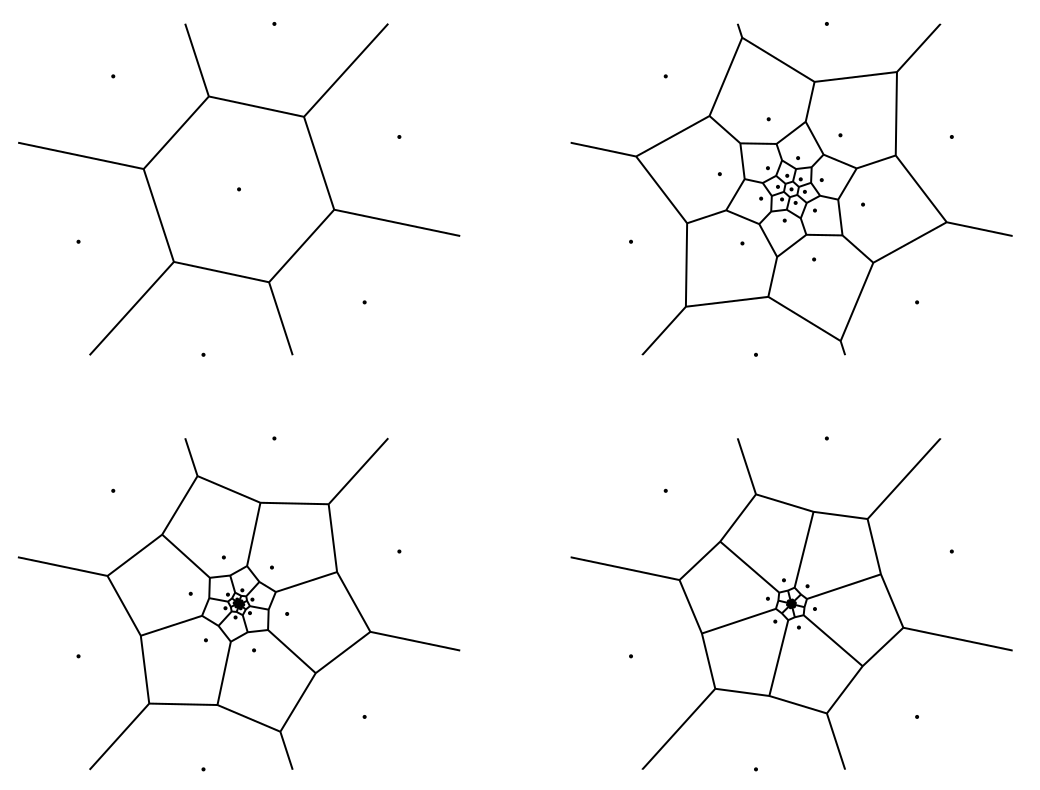
\includegraphics[width=.9\linewidth]{seed_placement.png}
    \caption{(From [\citen{VOISE}]) Effects of seed placement. Seeds are added to original VD (top right) recursively for three iterations, with $w_s$ = 0.25 (top right), $w_s$ = 0.5 (bottom left) and $w_s = 0.75$ (bottom right).}
    \label{seed-placement}
\end{figure}

The threshold $\chi_m$ is calculated using statistics on the set of homogeneity measures, $\{\chi(\mathcal{I}, s_i), s_i \in S\}$. The parameter $p_D$ is the proportion (or empirical probability) of VRs that are designated homogeneous on any given iteration, regardless of absolute values:
\begin{align}
	\text{P}\left(\chi(\mathcal{I}, s_i) < \chi_m\right) &= \frac{p_D}{100}
\end{align}
Because regions with high $\chi(\mathcal{I}, s_i)$ are split into regions with lower $\chi(\mathcal{I}, s_i)$, the denominator in eq. (\ref{homogeneity}) is monotonically decreacing as seeds are added. This has the effect of increacing $\chi(\mathcal{I}, s_i)$, increasing the strictness of the criteria. In this way, the features on the smaller length scales are picked up by VOISE. A $p_D$ of 70-80\%, with the median as merit function $\chi$, was found in [\citen{VOISE}] to extract only the features of highest contrast, whereas $p_D = 60-70\%$ results in better detection of smaller or more noisey features but worse detection of high contrast features.

In order to force convergence under these changing conditions, a minimum inter-seed distance is enforced, so that the process stops either when all VRs meet the homogeneity criteria or no more seeds can be legally added. At this point, the number of seeds is at a maximum and the image is at its most fragmented.

\subsubsection{Merging}

Once a VR is deemed inhomogeneous in the division phase, seeds are added with no reference to the underlying image but rather according to a set of fixed geometric rules. This means that redundancy is introduced, where seeds are added which create adjacent VRs that are similar to one another, which has the undesirable effect of feature splitting. In order to reverse this, redundant seeds must be removed algorithmically, and as such, all VRs are checked for the three conditions. In the following, $\mu_i$ can be any metric over all pixel intensities in a VR, chosen in [\citen{VOISE}] to be the median.
\begin{enumerate}[(a)]
	\item The VR must be homogeneous according to dynamic, statistically informed threshold analogous to that in the dividing phase:
	\begin{align}
			\chi(\mathcal{I}, s_i) < \chi_m
		\end{align}
		where
		\begin{align}
			\text{P}\left(\chi(\mathcal{I}, s_i) < \chi_m\right) &= \frac{p_M}{100}
		\end{align}
		$p_M$ is another parameter to be specified in the configuration of VOISE.
	\item There exist one or more seeds in the neighbourhood of the seed, $\{s_j \in \mathcal{N}(s_i)\}$, which are themselves homogeneous according to (a), and who's $\mu_j$ is lower than a set relative threshold $\Delta \mu$:
	\begin{align}
	\label{crit}
		|\mu_i - \mu_j| < \Delta \mu |\mu_i|
	\end{align}
	\item The fraction of the total perimeter ($\mathcal{P}$) of the VR which is shared with neighbours which are not similar according to eq. (\ref{crit}) ($\mathcal{L}$) is not above the stipulated threshold $\Delta \mathcal{H}$:
	\begin{align}
		\frac{\mathcal{L}}{\mathcal{P}} < \Delta \mathcal{H}
	\end{align}
\end{enumerate}
If all three conditions are met, the seed is removed and the VD is updated. The neighbouring cells then expand to include the pixels previously allocated to that seed. Because $\chi(\mathcal{I}, s_i)$ can only increase with the removal of seeds, condition (a) becomes more difficult to fulfill and so the merge phase concludes naturally when no more regions meet all three conditions. A more lax (larger) $p_M$ leads to less merging and therefore a representation with more seeds. A smaller value of $p_M$ gives a representation that more sparse, and results in a higher compression.

\subsubsection{Regularlisation}

Usually, the VRs obtained by the first three phases are irregular, with many acute angles and elongated polygons. In order to remedy this, an iterative process of seed movement can be employed, where each seed is moved to the centre of mass $\xi_i$ of the VR:
\begin{align}
	\xi_i &= \frac{\sum_{\textbf{p} \in \mathcal{R}(s_i)}\textbf{p} \rho(\textbf{p})}{\sum_{\textbf{p} \in \mathcal{R}(s_i)}\rho(\mathbf{p})}
\end{align}
Pixel intensity is used as the density function at pixel $\textbf{p}$, $\rho(\textbf{p})$, which is close to uniform within each VR after the previous three phases. Because the VD changes with the changing seed positions, this process must be iterative and stops either when the difference between seed position $s_i$ and $\xi_i$ is less than 1 for all $s_i \in S$ (because both seeds and the corresponding centres of mass are only defined in $\Omega$), or when a predetermined iteration limit is reached. After regularlisation, the process is complete.

\subsubsection{Applications of the VOISE algorithm}

The tesselations arrived at by VOISE have potential for the removal of errors caused by dust particles in images taken both on earth and from space telescopes, as long as a granularity is used that is high so as not to remove features but lower than the level required to be significantly affected by blemishes. In [\citen{VOISE2}], the authors of VOISE go on to use the seeds generated at the end of the division phase to estimate the disc parameters of planetary bodies, and in [\citen{VOISE3}], the seeds are used in Partitioning Around Metroids (PAM) clustering [\citen{PAM}] in the study of images of auroral emissions at the poles of Jupiter.
\textbf{Another possible use for VOISE include using the resulting seed coordinates as input vectors into machine learning algorithms, especially if images are labelled, which could provide a new approach to image recognition.}

\subsubsection{Previous Implementation of VOISE}

While the VOISE algorithm has been implemented previously [\citen{VOISE}], the method of VD recalculation is slower than is optimum. In that paper, VD calculation does borrow some techniques from SKIZ and is dynamic, but full integration of the SKIZ operator remains to be seen. While running time is not a concern when the number of images to be processed is low, if the VOISE algorithm is to be scaled up and its outputs used as input vectors for machine learning algorithms then this is no longer the case.

\subsection{The SKIZ Operator Algorithm}

VOISE requires recalculation of the VD after each iteration. In [\citen{skiz}], it is proven that adding and removing seeds only affects the VD in the neighbourhood of the added or removed seeds, a fact which is exploited to provide a dynamic algorithm which can be updated at a greatly reduced computational cost with respect to recalculating the entire VD. Using this, as well as a compiled language with a well optimised compiler (C++ with GCC), the VOISE algorithm can be made extremely fast.

\subsubsection{Data structures}

The SKIZ algorithm uses two matrix data structures, $\nu$ and $\lambda$, both of which have one element for each pixel. Their dimensions are the same as those of the image, but transposed; $\lambda_{ij}$ contains the ID of the closest seed for the pixel in the $i^{th}$ column of the $j^{th}$ row of the image, with $\nu_{ij}$ being equal to zero if the closest seed is unique, or 1 if there exist two or more closest seeds:
\begin{align}
\lambda_{ij} &= s \quad \text{s.t.}\quad d(p, s) \leq d(p, r) \quad \forall r \in S\textbackslash \{s\}\\
	\nu_{ij} &= \begin{cases}
	0 : d(p, \lambda_{ij}) < d(p, r) \quad \forall r \in S\textbackslash \{\lambda_{ij}\}\\
	1 : d(p, \lambda_{ij}) = d(p, r) \text{ for some } r \in S\textbackslash \{\lambda_{ij}\}
	\end{cases}
\end{align}
where seed $p$ has coordinates $(p_1, p_2) = (j, -i)$, so that a cartesian (bottom left, column-first) pixel coordinates match up with (top-left, row-first) matrix coordinates. From hereoanfter, the distance operator $d$ is assumed to be the squared Euclidian distance in $\mathbb{R}^2$ such that:
\begin{align}
	d(p, s) = (p_1 - s_1)^2 + (p_2 - s_2)^2
\end{align}
Squared distance is used because for $p, s \in \Omega$, $d(p, s)$ is a positive integer and we avoid the problems of floating point arithmetic. In C++, $\nu$ and $\lambda$ are stored as \verb|Eigen::Array| objects [\citen{Eigen}], which are stored internally arrays, bringing the associated efficiencies, but can be accessed using the \verb|()| operator by row and column index as well as a host of other useful features.
Another extremely important structure is the list of neighbouring cells $\mathcal{N}(s_i)$ (\verb|Nk| in code). In matlab, this is stored as a cell array, which in C++ is translated to as \verb|std::map<double, std::vector<double>>|, such that the vector of neighbouring seed IDs can be accessed using \verb|Nk.at(seed_id)|. At this point, it should be noted that for Matlab/C++ compatability, many variables (such as IDs) that would usually be stored as integers are stored as doubles. We now have the required data structures in place for efficient calculation of VDs.

\subsubsection{Checking Voronoi Region Bounds (getRegion.cpp)}

Imagine that a seed $s$* is added to a VD, and that there is a pixel for which we would like to know the associated VR. One way of checking would be to compare $d(p, s_i) \quad \forall s_i \in S_k \cup \{s\text{*}\}$ and choosing $s_i$ with the lowest distance, however that operation would require the calculation of $\left(|S_k| + 1\right)$ distances and $\left(|S_k| + 1\right)$ comparisons.

Instead, it is proven in [\citen{skiz}, sec. 2.2] that checking if a pixel is within a VR $\mathcal{R}(s)$ can be reduced to checking two inequalities. In sec. 2 of that paper, it is proven that the half-plane $H$ which represents points that are closer to point $p$ than $q$ can be represented by an inequality:
\begin{align}
\label{halfplanes}
	H(p, q) &= \left\{ x \in \mathbb{R}^2 : d(x, p) < d(x, q) \right\} = \left\{x \in \mathbb{R}^2 : ax_1 + bx_2 > c \right\}\\
	\text{where} \quad a &= p_1 - q_1 \nonumber \\ 
	b &= p_2 - q_2 \nonumber \\ 
	c &= (p_1^2 + p_2^2 - q_1^2 - q_2^2)/2 \nonumber
\end{align}
It is also proven that $\mathcal{R}(s_i)$ is defined only by the intersection of halfplanes between $s_i$ and its neighbours $\mathcal{N}(s_i)$; The number of inequalities of the form (\ref{halfplanes}) is therefore limited by $\left(|\mathcal{N}(s_i)\right|$. If we are finding whether a point is in the halfplane $H(s_i, r), r \in \mathcal{N}(s_i)$, eq. (\ref{halfplanes}) can be rearranged into one of the following inequalities, depending on the values of the coordinates $s_1, s_2, r_1$ and $r_2$:
\begin{align}
\label{getRegion}
	s_1 - r_1 : \begin{cases}
	= 0 : \begin{cases}
	s_2 > r_2 : i < \frac{s_2 + r_2}{2}\\
	s_2 < r_2 : i > \frac{s_2 + r_2}{2}
	\end{cases}\\
	< 0 : \quad j < \frac{s_1^2 + s_2^2 - r_1^2 - r_2^2}{2(p_1-q_1)}-(s_2 - r_2)i\\
	> 0 : \quad j > \frac{s_1^2 + s_2^2 - r_1^2 - r_2^2}{2(p_1-q_1)} - (s_2 - r_2)i
	\end{cases}
\end{align}
The most common of these are where $s_1 \neq r_1$, which gives a set of upper and lower bounds on $j$ for each row $i$. If the value of $j$ of a pixel on row $i$ is above the maximum lower and below the minimum upper bounds, then it belongs to the VR of the seed $s$. Where $s_1 = r_1$, $j$ cancels and the condition is soley based on the value of $i$. At this point, we have an $I \times 2$ matrix of lower and upper bounds for each row, which any pixel can be checked against for membership of the VR, where $I$ is the total number of rows.

\subsubsection{Adding a seed (addSeed.cpp)}

The subscript $k$ is used here to denote iteration number - it increments whenever a seed is added or removed. $\mathcal{N}_k$ is the map of neighbour relationships at iteration $k$, with $S_k$ defined similarly. When a seed $s$* is added, $\lambda_{ij}$ and $\nu_{ij}$ change according to:
\begin{align}
	\left[\lambda_{ij, k+1}, \nu_{ij, k+1}\right] = \begin{cases}
		\left[\lambda_{ij, k}, \nu_{ij, k}\right] &\text{ if } d(p, \lambda_{ij, k}) < d(p, s\text{*})\\
		\left[\lambda_{ij, k}, 1 \right] &\text{ if } d(p, \lambda_{ij, k}) = d(p, s\text{*})\\
		\left[ s\text{*}, 0 \right] &\text{ if } d(p, \lambda_{ij, k}) > d(p, s\text{*})
	\end{cases}
\end{align}
If we know $\mathcal{N}_{k+1}(s$*$)$, we can use the inequalities found by eq. (\ref{getRegion}) to only check values of $\lambda$ and $\nu$ that are in $\mathcal{R}(s$*$)$, minimising the number of comparisons. We must therefore first find the new neighbour relationships of all seeds, $\mathcal{N}_{k+1}(s_i), s_i \in S_k \cup s$*.

\subsubsection{Finding $\mathcal{N}_{k+1}$}

The approach to finding $\mathcal{N}_{k+1}$ described in [\citen{skiz}] borrows from the \textit{incremental method} [\citen{green_sibson_1978}], and involves building up $\mathcal{N}_{k+1}(s$*$)$ by finding boundaries of $\mathcal{R}(s$*$)$. Beginning with $\mathcal{N}_{k+1}(s$*$) = \{\lambda\}$ where $\lambda$ is the closest seed in $S_k$ to the point now occupied by $s$*.




\newpage
\appendix
\bibliographystyle{plain}
\bibliography{bibfile}

\end{document}